\section{Secure Programming (mobile)}
\subsection{Demo App 1 - Insecure Data Storage}
\subsubsection{App description}
With this app a user has to perform a simple login to access another screen (see figure \ref{fig:app0}). Since the login mechanism is mocked, both username and password are hard-coded (username: \textit{sse} / password: \textit{topsecret}). The app features the functionality to store entered login information, which is the part of this application that can be exploited.

\begin{figure}[htb!]
	\centering
	\begin{subfigure}{.3\textwidth}
  		\centering
  		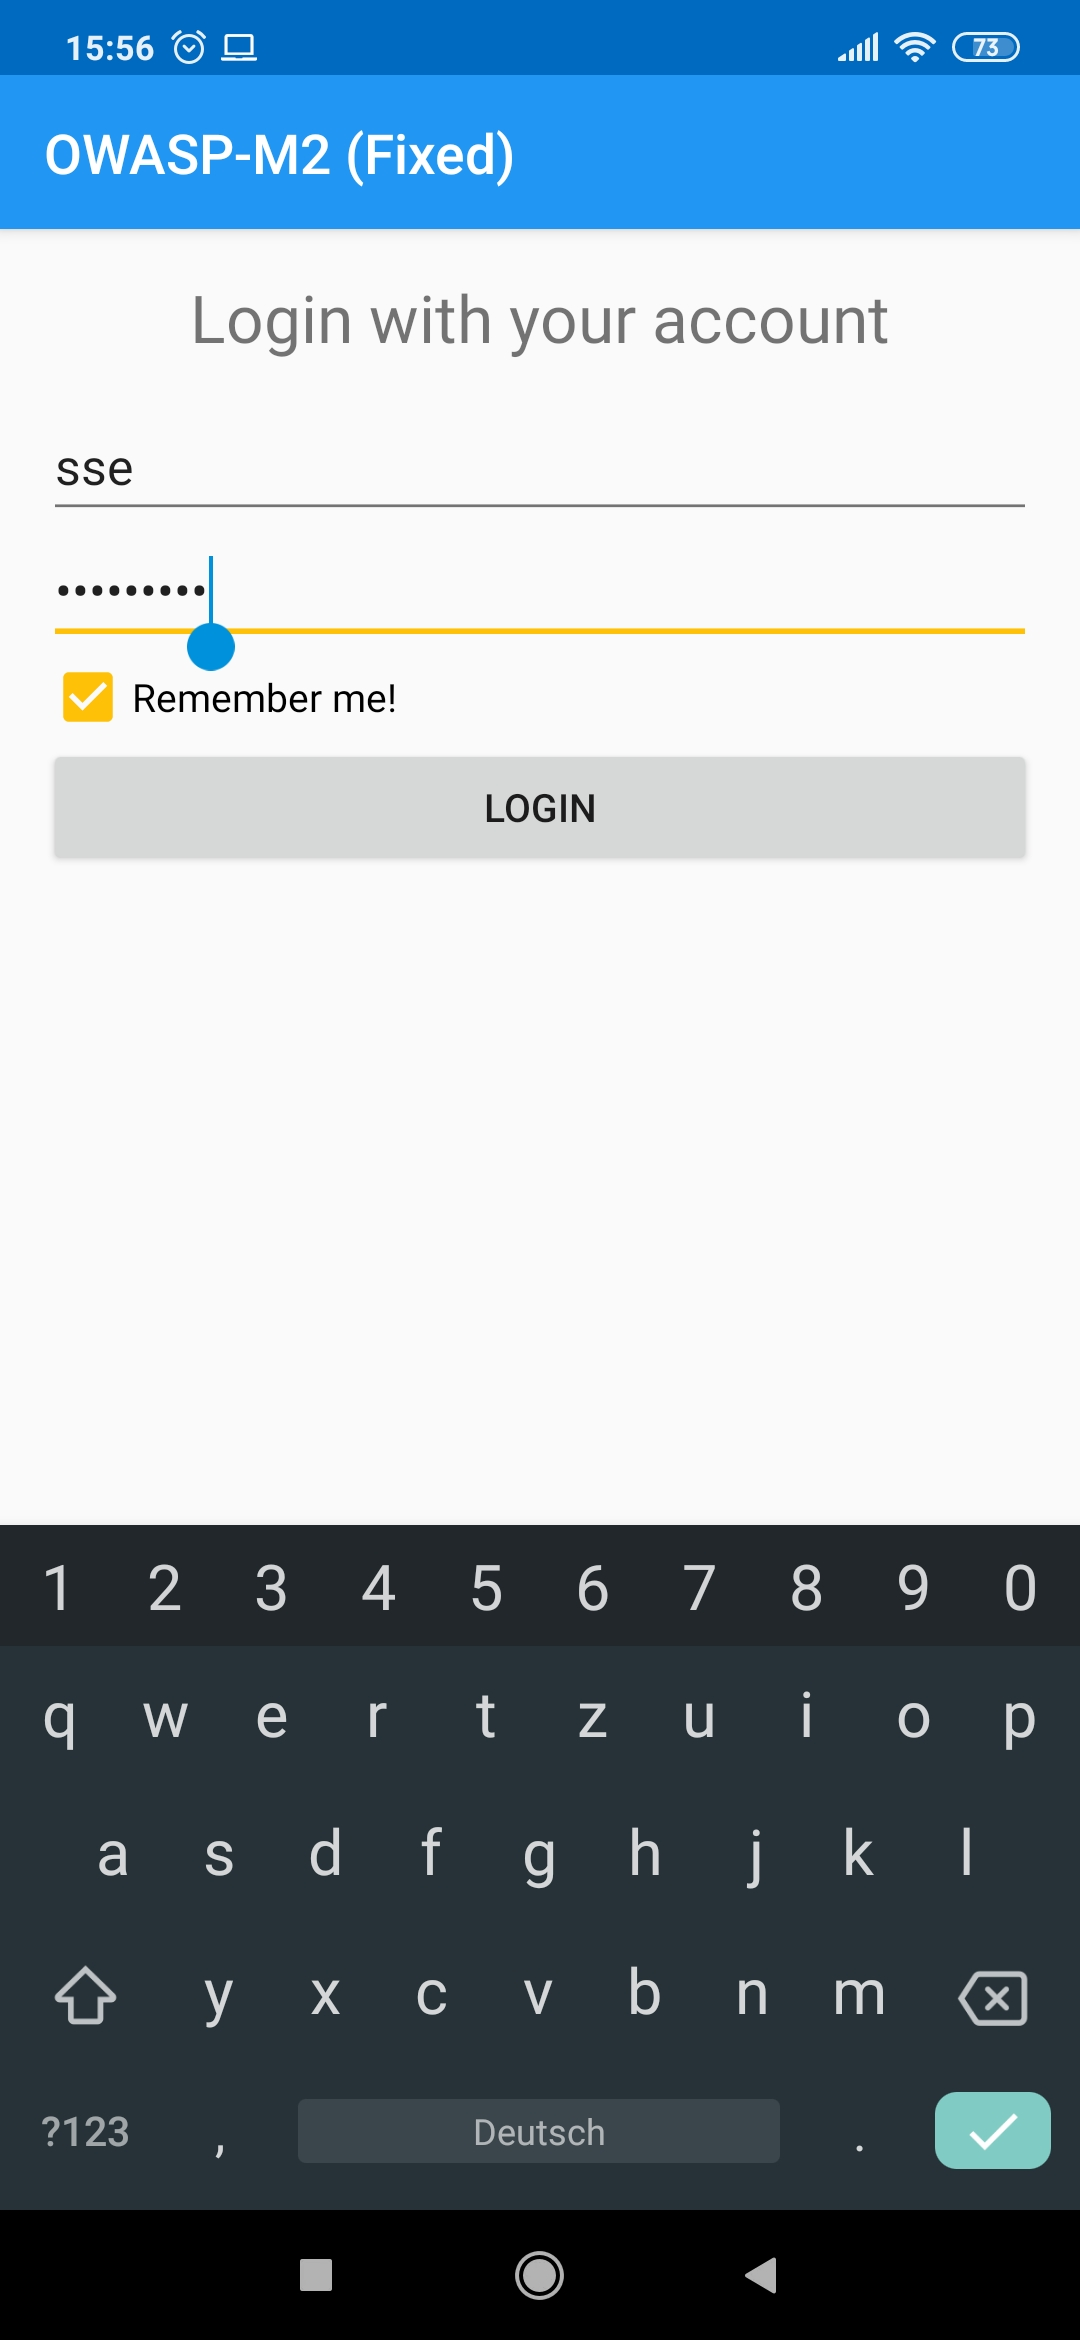
\includegraphics[width=\linewidth]{imgs/secure_mobile_programming/app0_login_form_filled.jpg}
  		\caption{Login screen}
	\end{subfigure}
	\begin{subfigure}{.3\textwidth}
  		\centering
  		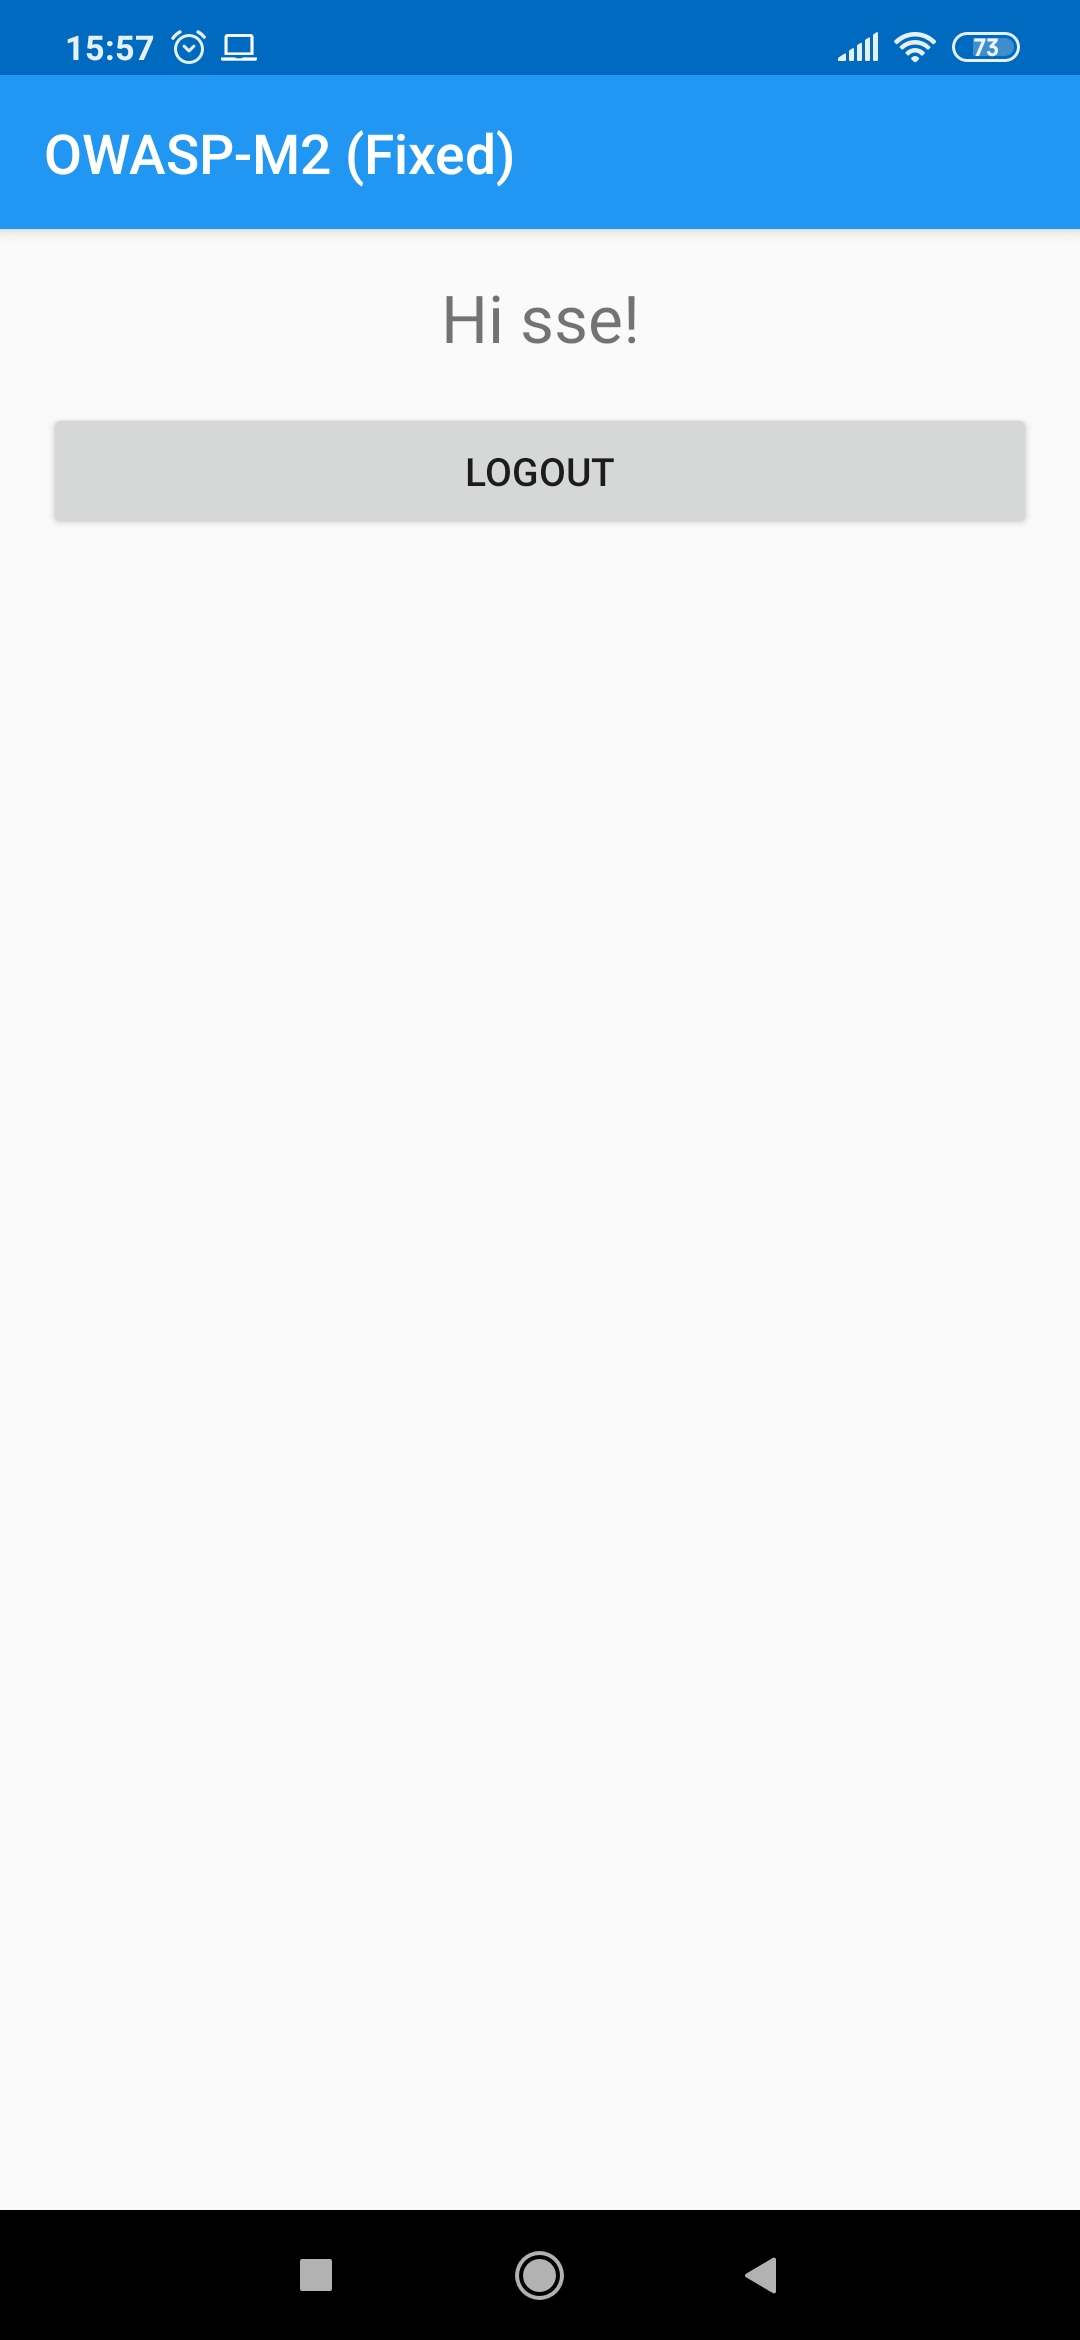
\includegraphics[width=\linewidth]{imgs/secure_mobile_programming/app0_logged_in.jpg}
  		\caption{Logged-in screen}
	\end{subfigure}
	\caption{Screens of the first app}
	\label{fig:app0}
\end{figure}


\subsubsection{Vulnerability}
\paragraph{Theoretical Background:}
Insecure data storage is a common problem with mobile apps and takes the second place in the OWASP mobile top ten. It implies that storing sensitive data in an insecure way allows attackers or malware to access it without the users or the apps permission.

The leakage of sensitive app data can lead to privacy violation, identity theft or even fraud.

\paragraph{Location of the Vulnerability:} 
In the original version of the app, the vulnerability is located in the \texttt{ExternalAuthenticationStorageManager} class. This class uses Androids external storage to save authentication data (username and password) in a JSON file. The external storage on Android can be accessed by the user and every other app, which makes it the worst place to store sensitive data.

\paragraph{Possible Solutions:} Android provides several ways to store data. Three options that can not be accessed by a normal Android user or other apps are:
\begin{itemize}
	\item Internal storage
	\item App preferences
	\item Database
\end{itemize}
These should be the first options when it comes to saving sensitive data. The only way to access these storage options is when an app has superuser privileges. Therefore, sensitive data should also be encrypted properly (see section \ref{sec:app1}).


\subsubsection{Exploitation}
\paragraph{How to exploit this App:}
As mentioned before, the unpatched version of this app uses Androids external storage to save the users credentials. If a user has checked the 'Remember me!' checkbox, a JSON file gets created that contains both the username and the password when a successful login was performed. This file can then be accessed and edited by every other app or the user him- or herself. It can be found in \textit{/storage/emulated/0/Android/data/at.ac.tuwien.sse.owaspm2/files/auth-data.json}.

\paragraph{How the patched version is more secure:}
The patched version uses app preferences, shared preferences to be more exact, to save authentication data. Instead of \texttt{External AuthenticationStorageManager} it now uses the \texttt{SharedPrefsAuthenticationStorage Manager} class (both are implementing the same interface, \texttt{IAuthenticationStorage Manager}, which made the patching process much easier).

Shared preferences are key-value pairs within the internal storage, so only the app itself can access them. To make this even more secure, instead of saving both the username and the password, only the username and a session id gets stored. 



\subsection{Demo App 2 - Insufficient Cryptography}\label{sec:app1}
\subsubsection{App description}
With this app a user can enter his or her credit card information and store them on his or her phone. To save and encrypt the information, a password is required. After encryption, the credit card data is stored in the internal storage so that only this app has access to it (like with the first app, as long as we can assume that other apps don't have superuser privileges).

To decrypt and show the credit card information, a user has to provide the password that he or she entered during the creation of the credit card entry. Stored credit card information can also be deleted.

\begin{figure}[htb!]
	\centering
	\begin{subfigure}{.3\textwidth}
  		\centering
  		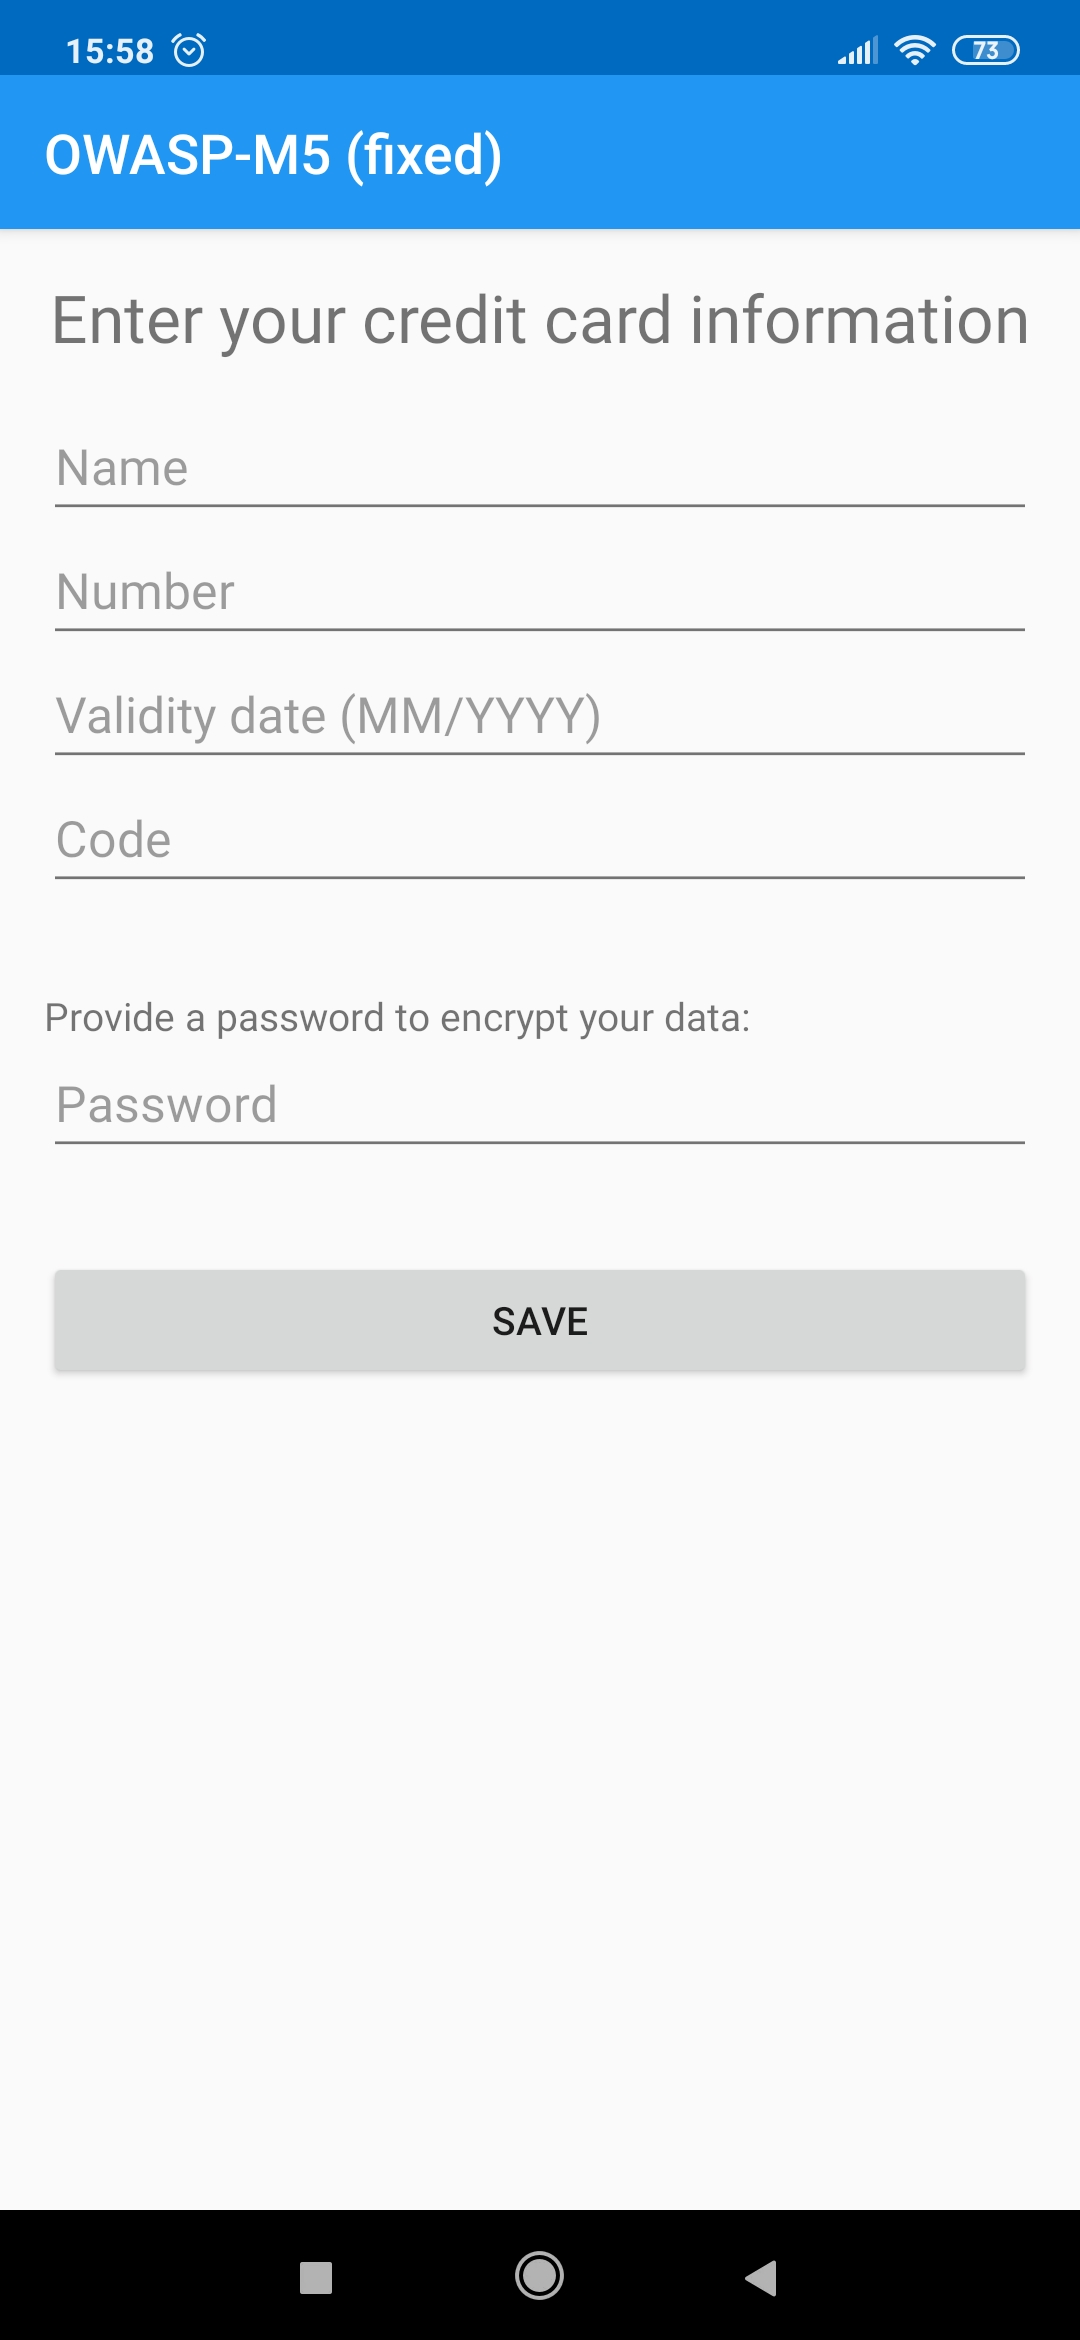
\includegraphics[width=\linewidth]{imgs/secure_mobile_programming/app1_credit_card_form_empty.jpg}
  		\caption{Credit card form}
	\end{subfigure}
	\begin{subfigure}{.3\textwidth}
  		\centering
  		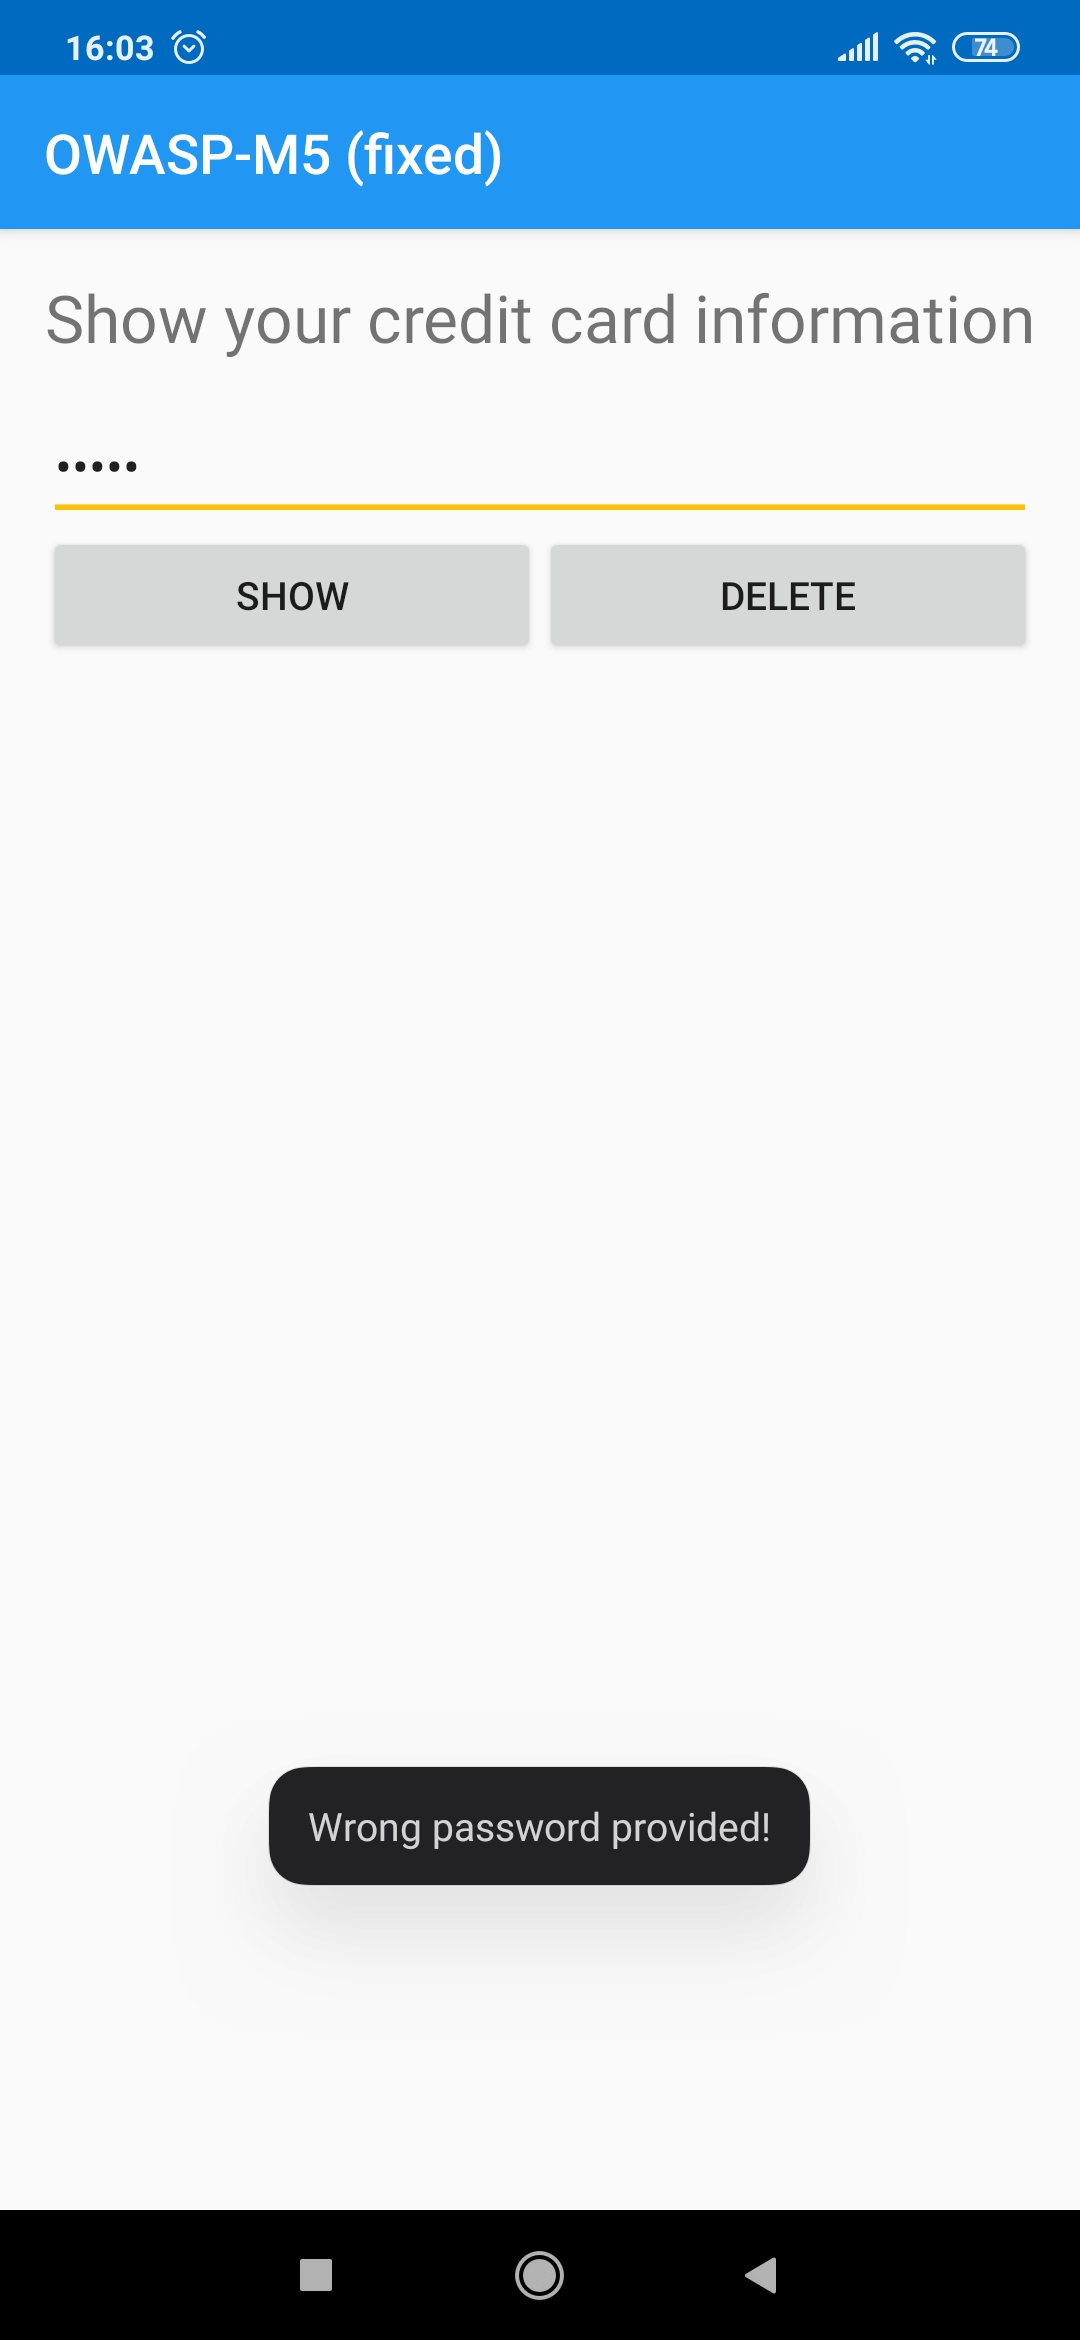
\includegraphics[width=\linewidth]{imgs/secure_mobile_programming/app1_credit_card_info_wrong_password.jpg}
  		\caption{Wrong password}
	\end{subfigure}
	\begin{subfigure}{.3\textwidth}
  		\centering
  		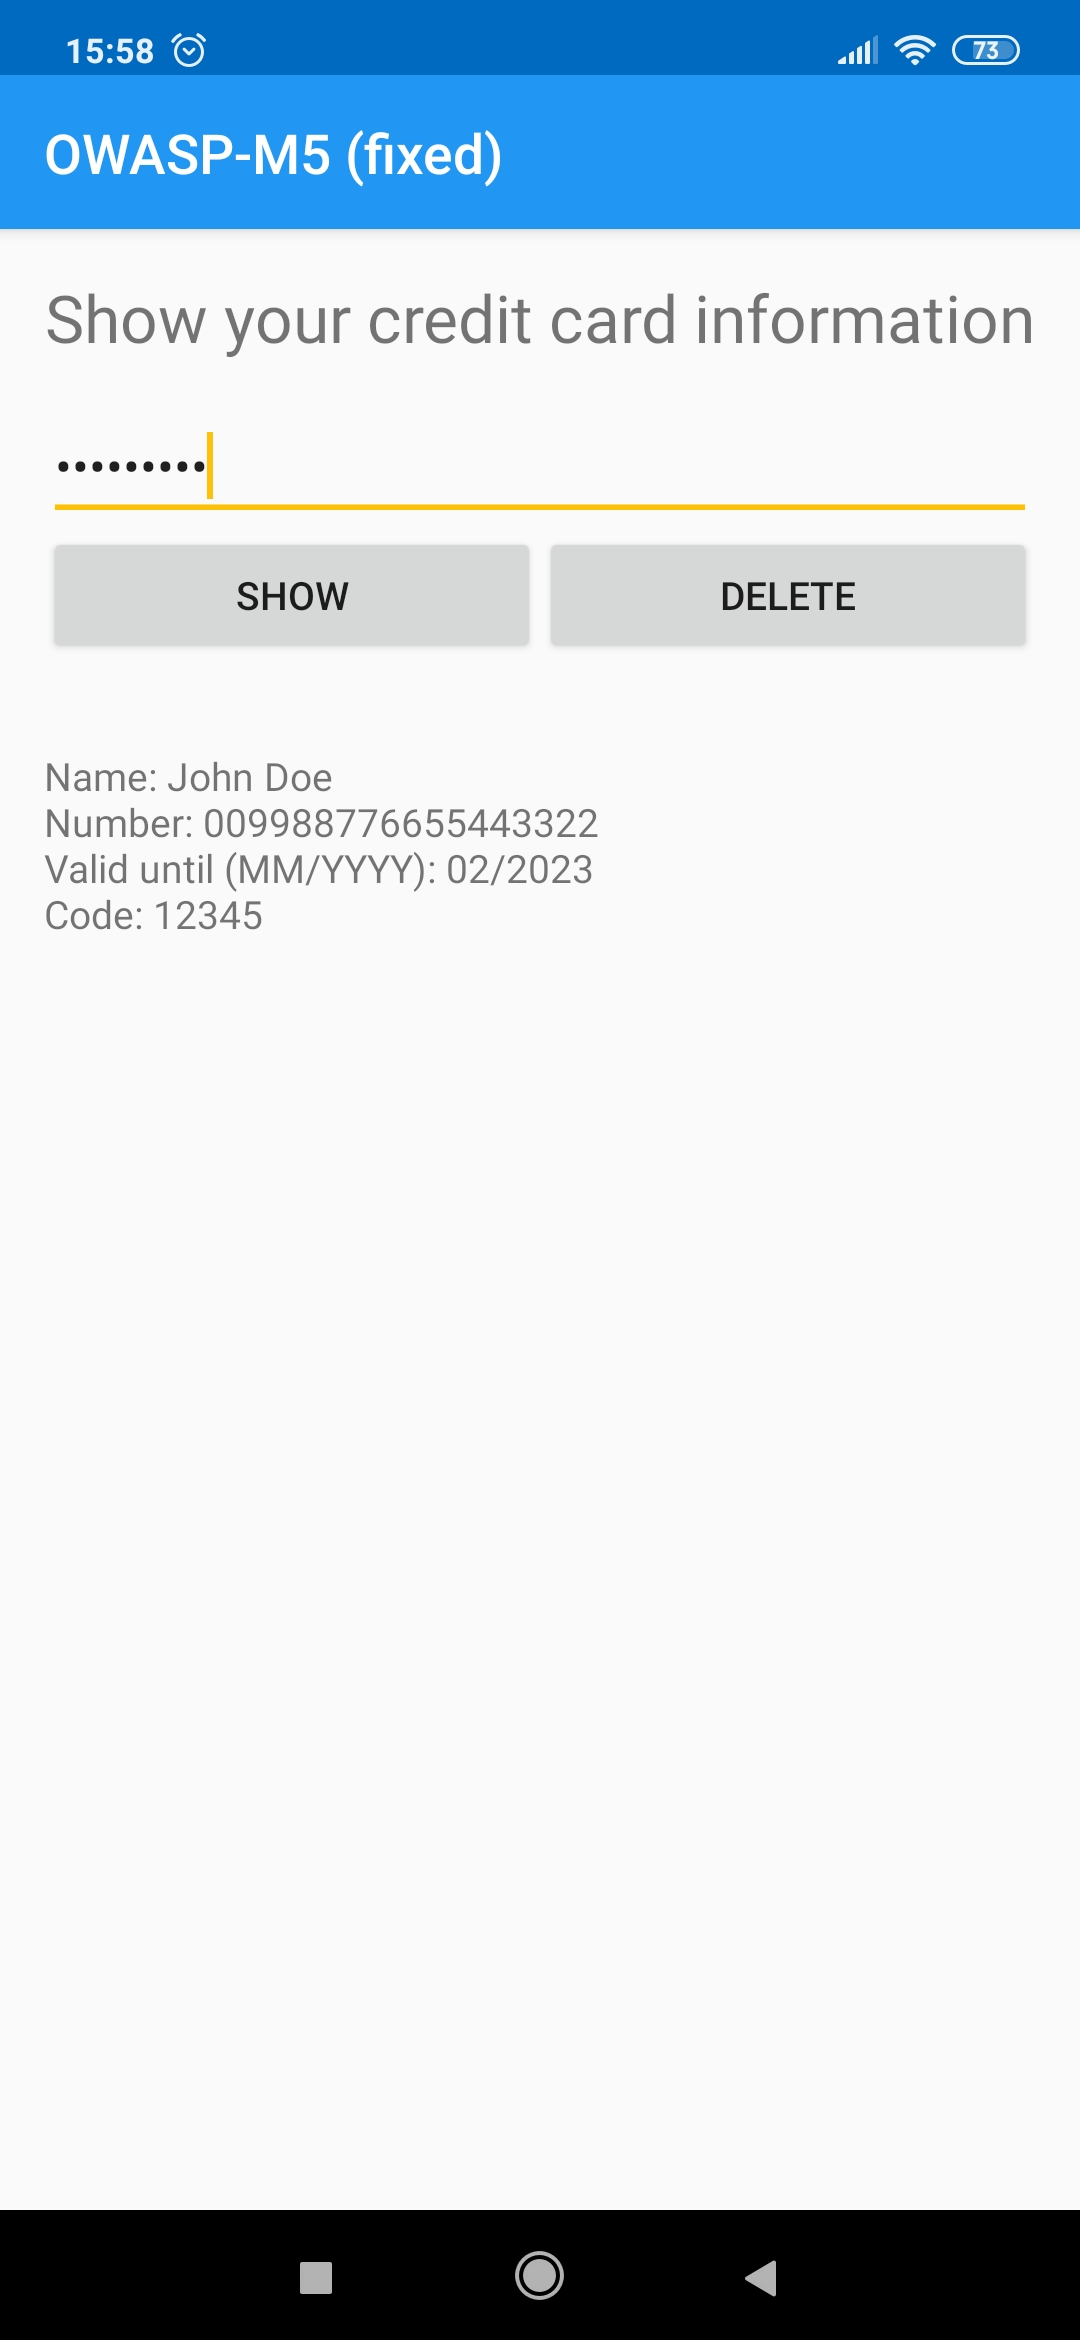
\includegraphics[width=\linewidth]{imgs/secure_mobile_programming/app1_credit_card_info_shown.jpg}
  		\caption{Correct password}
	\end{subfigure}
	\caption{Screens of the second app}
	\label{fig:app1}
\end{figure}


\subsubsection{Vulnerability}
\paragraph{Theoretical Background:}
Insufficient cryptography takes the fifth place in the OWASP mobile top ten. It occurs when data, especially sensitive information, is improperly or not at all encrypted and can be easily decrypted. 

Improperly encrypted means that insecure or deprecated algorithms are used, that keys are poorly managed or even custom encryption algorithms are used. Like with insecure data storage, this can lead to privacy violation or information theft.

\paragraph{Location of the Vulnerability:} \label{sec:app1-vulnerability}
The vulnerability of this app is located in the \texttt{OwnEncryption Manager} class. As the name implies, it uses a custom encryption method which is by no means secure. 

The algorithm iterates over each character in the plaintext and adds the corresponding password character and the counter variable to it (see listing \ref{lst:app0}). The encrypted message can then be decrypted by doing the exact opposite, i.e. subtracting each password character and the counter variable from the cipher text.

\begin{lstlisting}[language=Java, label={lst:app0}]
for (int i = 0; i < dataArray.length; i++) {
    cipherArray[i] = dataArray[i] + passwordArray[i % passwordArray.length] + i;
}
\end{lstlisting}


\paragraph{Possible Solutions:}
The solutions to this cryptography-problem are pretty simple:
\begin{itemize}
	\item Usage of well-established and strong cryptographic algorithms (like the ones defined in the Android developer cryptography guide).
	\item Not storing sensitive data on the device.
\end{itemize}


\subsubsection{Exploitation}
\paragraph{How to exploit this App:}
Like mentioned before, the data in the unpatched version is stored in the internal storage, which makes it harder to obtain. But if an attacker accomplishes to find and open the file that contains the encrypted data, he or she can easily identify the custom algorithm and decrypt the data to get access to the saved credit card information (see section \ref{sec:app1-vulnerability}).


\paragraph{How the patched version is more secure:}
The patched version uses \texttt{AESEncryptionManager} instead of the \texttt{OwnEncryptionManager} (like in the first app, both are implementing the same interface, \textbf{IEncryptionManager}).

This class follows the Android developer recommendations for encryption. It first generates in 1000 iterations of the \textit{Password-Based Key Derivation Function 2 (PBKDF2)} a key with a random salt and the entered password. Then, for encryption and decryption, it uses the \textit{Advanced Encryption Standard (AES)} in \textit{Galois/Counter Mode (GCM)} mode. Finally the resulting byte array gets stored as a Base64 encoded string in the output file within Android's internal storage. The random salt and the initialization vector are both saved as shared preferences in the internal storage as well.
